\documentclass[ngerman,hyperref={pdfpagelabels=false}]{beamer}

% -----------------------------------------------------------------------------

\graphicspath{{images/}}

% -----------------------------------------------------------------------------

\usetheme{KIT}

\setbeamercovered{transparent}
%\setbeamertemplate{enumerate items}[ball]

\newenvironment<>{KITtestblock}[2][]
{\begin{KITcolblock}<#1>{#2}{KITblack15}{KITblack50}}
{\end{KITcolblock}}

\usepackage[ngerman,english]{babel}
\usepackage[utf8]{inputenc}
\usepackage[TS1,T1]{fontenc}
\usepackage{array}
\usepackage{multicol}
\usepackage[absolute,overlay]{textpos}
\usepackage{beamerKITdefs}
\usepackage{caption}
\usepackage{verbatim}

%----------------------------------
% thomi fa list implementation
%----------------------------------

\newlist{falist}{enumerate}{2}
\setlist[falist,1]{label={/FA\arabic{falisti}\arabic{falistii}/},align=left,labelwidth=17pt,labelsep=3pt,leftmargin=20pt}
\setlist[falist,2]{label={/FA\arabic{falisti}\arabic{falistii}/}}%,align=left,labelwidth=17pt,labelsep=3pt,leftmargin=0pt}

\usepackage{chngcntr}
\counterwithin{falistii}{falisti}

\newlist{pdlist}{enumerate}{2}
\setlist[pdlist,1]{label={/PD\arabic{pdlisti}\arabic{pdlistii}/},align=left,labelwidth=17pt,labelsep=3pt,leftmargin=20pt}
\setlist[pdlist,2]{label={/PD\arabic{pdlisti}\arabic{pdlistii}/}}%,align=left,labelwidth=17pt,labelsep=3pt,leftmargin=0pt}
\counterwithin{pdlistii}{pdlisti}

\newlist{nflist}{enumerate}{2}
\setlist[nflist,1]{label={/NF\arabic{nflisti}\arabic{nflistii}/},align=left,labelwidth=17pt,labelsep=3pt,leftmargin=20pt}
\setlist[nflist,2]{label={/NF\arabic{nflisti}\arabic{nflistii}/}}%,align=left,labelwidth=17pt,labelsep=3pt,leftmargin=0pt}
\counterwithin{nflistii}{nflisti}

\newlist{telist}{enumerate}{2}
\setlist[telist,1]{label={/T\arabic{telisti}\arabic{telistii}/},align=left,labelwidth=17pt,labelsep=3pt,leftmargin=20pt}
\setlist[telist,2]{label={/T\arabic{telisti}\arabic{telistii}/}}%,align=left,labelwidth=17pt,labelsep=3pt,leftmargin=0pt}
\counterwithin{telistii}{telisti}

\pdfpageattr {/Group << /S /Transparency /I true /CS /DeviceRGB>>}	%required to prevent color shifting withd transparent images


\title{Kolloquium Qualitätssicherung RetroMachines}
\subtitle{Team B (RetroFactory)}

\author[Team B (RetroFactory)]{Team B (RetroFactory)}
\institute{Institut für Programmierparadigmen}

\TitleImage[width=\titleimagewd,height=\titleimageht]{titel}

\KITinstitute{Institut f\"ur Programmierparadigmen}
\KITfaculty{Fakult\"at f\"ur Informatik}

% -----------------------------------------------------------------------------

\begin{document}
\setlength\textheight{7cm} %required for correct vertical alignment, if [t] is not used as documentclass parameter


% title frame
\section{Deckblatt}
\begin{frame}
  \maketitle
\end{frame}

\begin{frame}
\frametitle{Tests}
\framesubtitle{Instruction Coverage}
{
  \centering
  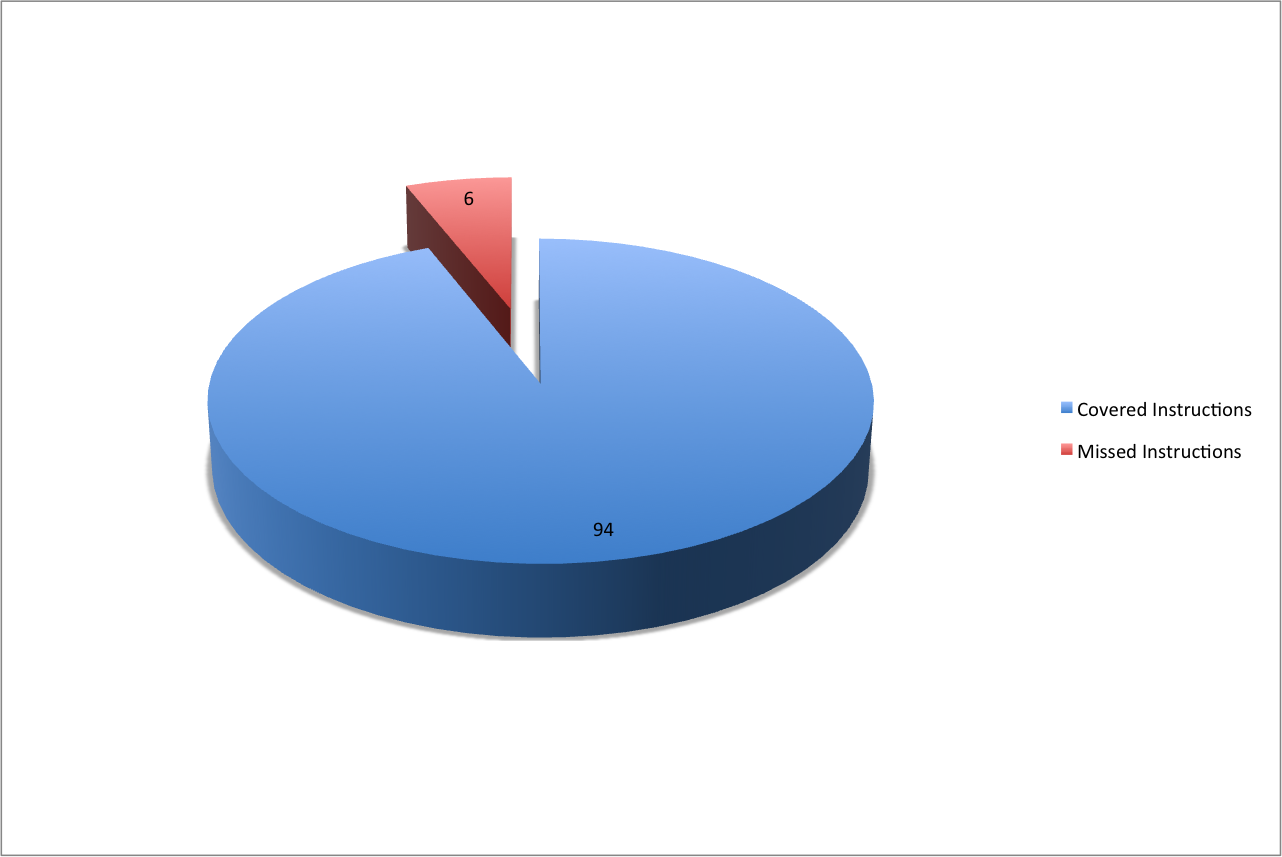
\includegraphics[scale=0.3]{instructions.png}
  \par
}
\end{frame}

\begin{frame}
  \frametitle{Tests}
  \framesubtitle{Branch Coverage}
  {
    \centering
    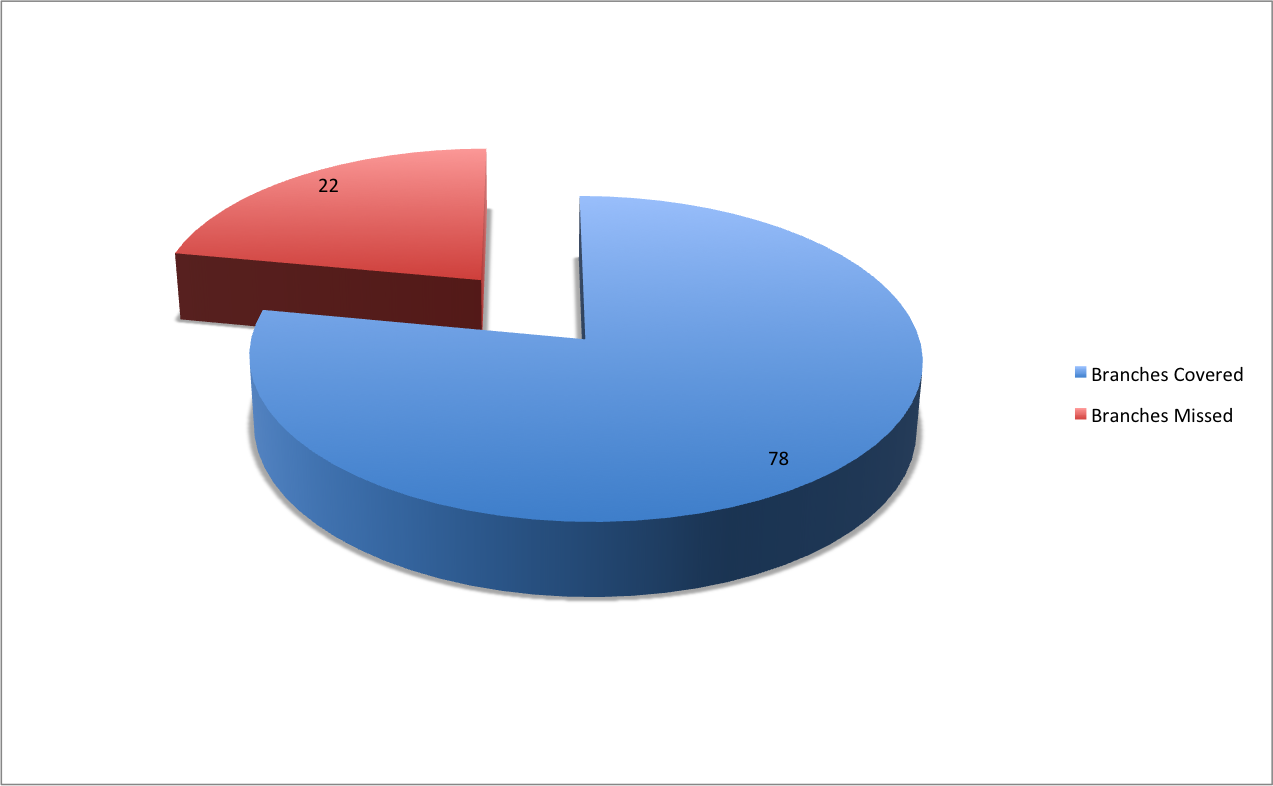
\includegraphics[scale=0.3]{branches.png}
    \par
  }
\end{frame}

\begin{frame}
  \frametitle{Tests}
  \framesubtitle{Tabellarische Übersicht}

  \begin{tabular} { | l | c | c | c | c | c | c | }
  \hline
  \textbf{Package} & \textbf{IC} & \textbf{BC} \\
  \hline
  Insgesamt & 94\% & 76\% \\
  \hline
  com.retroMachines & 100\% & 75\% \\
  \hline
  com.retroMachines.data & 100\% & 100\%  \\
  \hline
  com.retroMachines.data.models & 100\% & 100\% \\
  \hline
  com.retroMachines.game & 93\% & 72\% \\
  \hline
  com.retroMachines.game.controllers & 98\% & 89\% \\
  \hline
  com.retroMachines.game.gameelements & 96\% & 91\% \\
  \hline
  com.retroMachines.ui & 100\% & 100\% \\
  \hline
  com.retroMachines.ui.screens & 100\% & 100\% \\
  \hline
  com.retroMachines.ui.screens.game & 89\% & 56\% \\
  \hline
  com.retroMachines.ui.screens.menus & 99\% & 85\% \\

  \hline
  com.retroMachines.util & 100\% & 67\% \\
  \hline
  com.retroMachines.util.lambda & 85\% & 70\% \\
  \hline
\end{tabular}
\end{frame}

\begin{frame}
    \frametitle{Tests}
    \framesubtitle{Weiterführendes}
    \begin{itemize}
        \item Monkey Testing
        \item monkeyrunner
        \item CodePro AnalytiX
        \item FindBugs
        \item Codeumstrukturierung
    \end{itemize}
\end{frame}

\begin{frame}
  \frametitle{Änderungen}
  \framesubtitle{Gefundene Bugs}
  Es wurden folgende Bugs im Code gefunden:
  \begin{itemize}
      \item Löschen des aktiven Profils
      \item Fehler beim Starten des Levels
      \item Erstellen von Profilen (Groß- und Kleinschreibung)
  \end{itemize}
  Alle drei Fehler konnten behoben werden.
\end{frame}

\begin{frame}
    \frametitle{Änderungen}
    \framesubtitle{Feedback von Nutzern}
    {
        \LARGE
        \textit{
            ``Die Tutorialhinweise sind zu unverständlich!''
        }
    }
    \begin{flushright}
        Ein sonst zufriedener Spieler
    \end{flushright}
\end{frame}

\begin{frame}
    \frametitle{Änderungen}
    \framesubtitle{Feedback von Nutzern}
    \begin{itemize}
        \item Aufspaltung von Grafiken in Einzelne.
        \item Hinzufügen weiterer Grafiken.
        \item Einfügen eines Knopfes zum Zurücksetzen der Hinweise.
    \end{itemize}
\end{frame}

\begin{frame}
    \frametitle{Änderungen}
    \framesubtitle{Weiterführendes}
    \begin{itemize}
        \item Kleinere Änderungen am Pflichtenheft, vornehmlich durch Umstrukturierungen der Menüstruktur
        \item Einfügen von Fehlermeldungen und Hinweisen
        \item Optimierung der UI Elemente
    \end{itemize}
\end{frame}


\end{document}
